\appendix[A short overview of our development]
In this appendix we succintly describe the contents of each file. In
the next page we include a dependency graph of our formalization. The
theories on a grayish background are directly from Paulson; we
highlight with light-blue/cyan those of Paulson that we modified. We
have developed from scratch the rest, in white.

\begin{description}
\item[\texttt{Nat\_Miscelanea}]Miscelaneous results for naturals, mostly
  needed for renamings.
\item[\texttt{Renaming}] Renaming of internalized formulas, see
  Section \ref{sec:renaming}.
\item[\texttt{Pointed\_DC}] A new choice principle.
\item[\texttt{Recursion\_Thms}] Enhancements about recursively defined
  functions.
\item[\texttt{Forcing\_Notions}] Definition of Posets with maximal
  element, filters, dense sets. Proof of Rasiowa-Sikorski.
\item[\texttt{Forcing\_Data}] Definition of the locales:
  \begin{inlinelist}
  \item \texttt{M\_ZF} satisfaction of axioms; and 
  \item \texttt{Forcing\_Data} extending the previous one with
    \texttt{Forcing\_notion}, transitivity, and being countable.
  \end{inlinelist}
\item[\texttt{Interface}] Instantiation of locales \texttt{M\_trivial}
  and \texttt{M\_basic} for every instance of \texttt{Forcing\_Data}.
\item[\texttt{Names}] Definitions of $\chk$, $\val$, and the generic
  extension. Various results about them.
\item[\texttt{Forcing\_Theorems}] Specification of fundamental
  theorems of forcing, see Section~\ref{sec:forcing}.
\item[\texttt{*\_Axiom}] Proof of the satisfaction of the
  corresponding axiom in the generic extension.
\end{description}

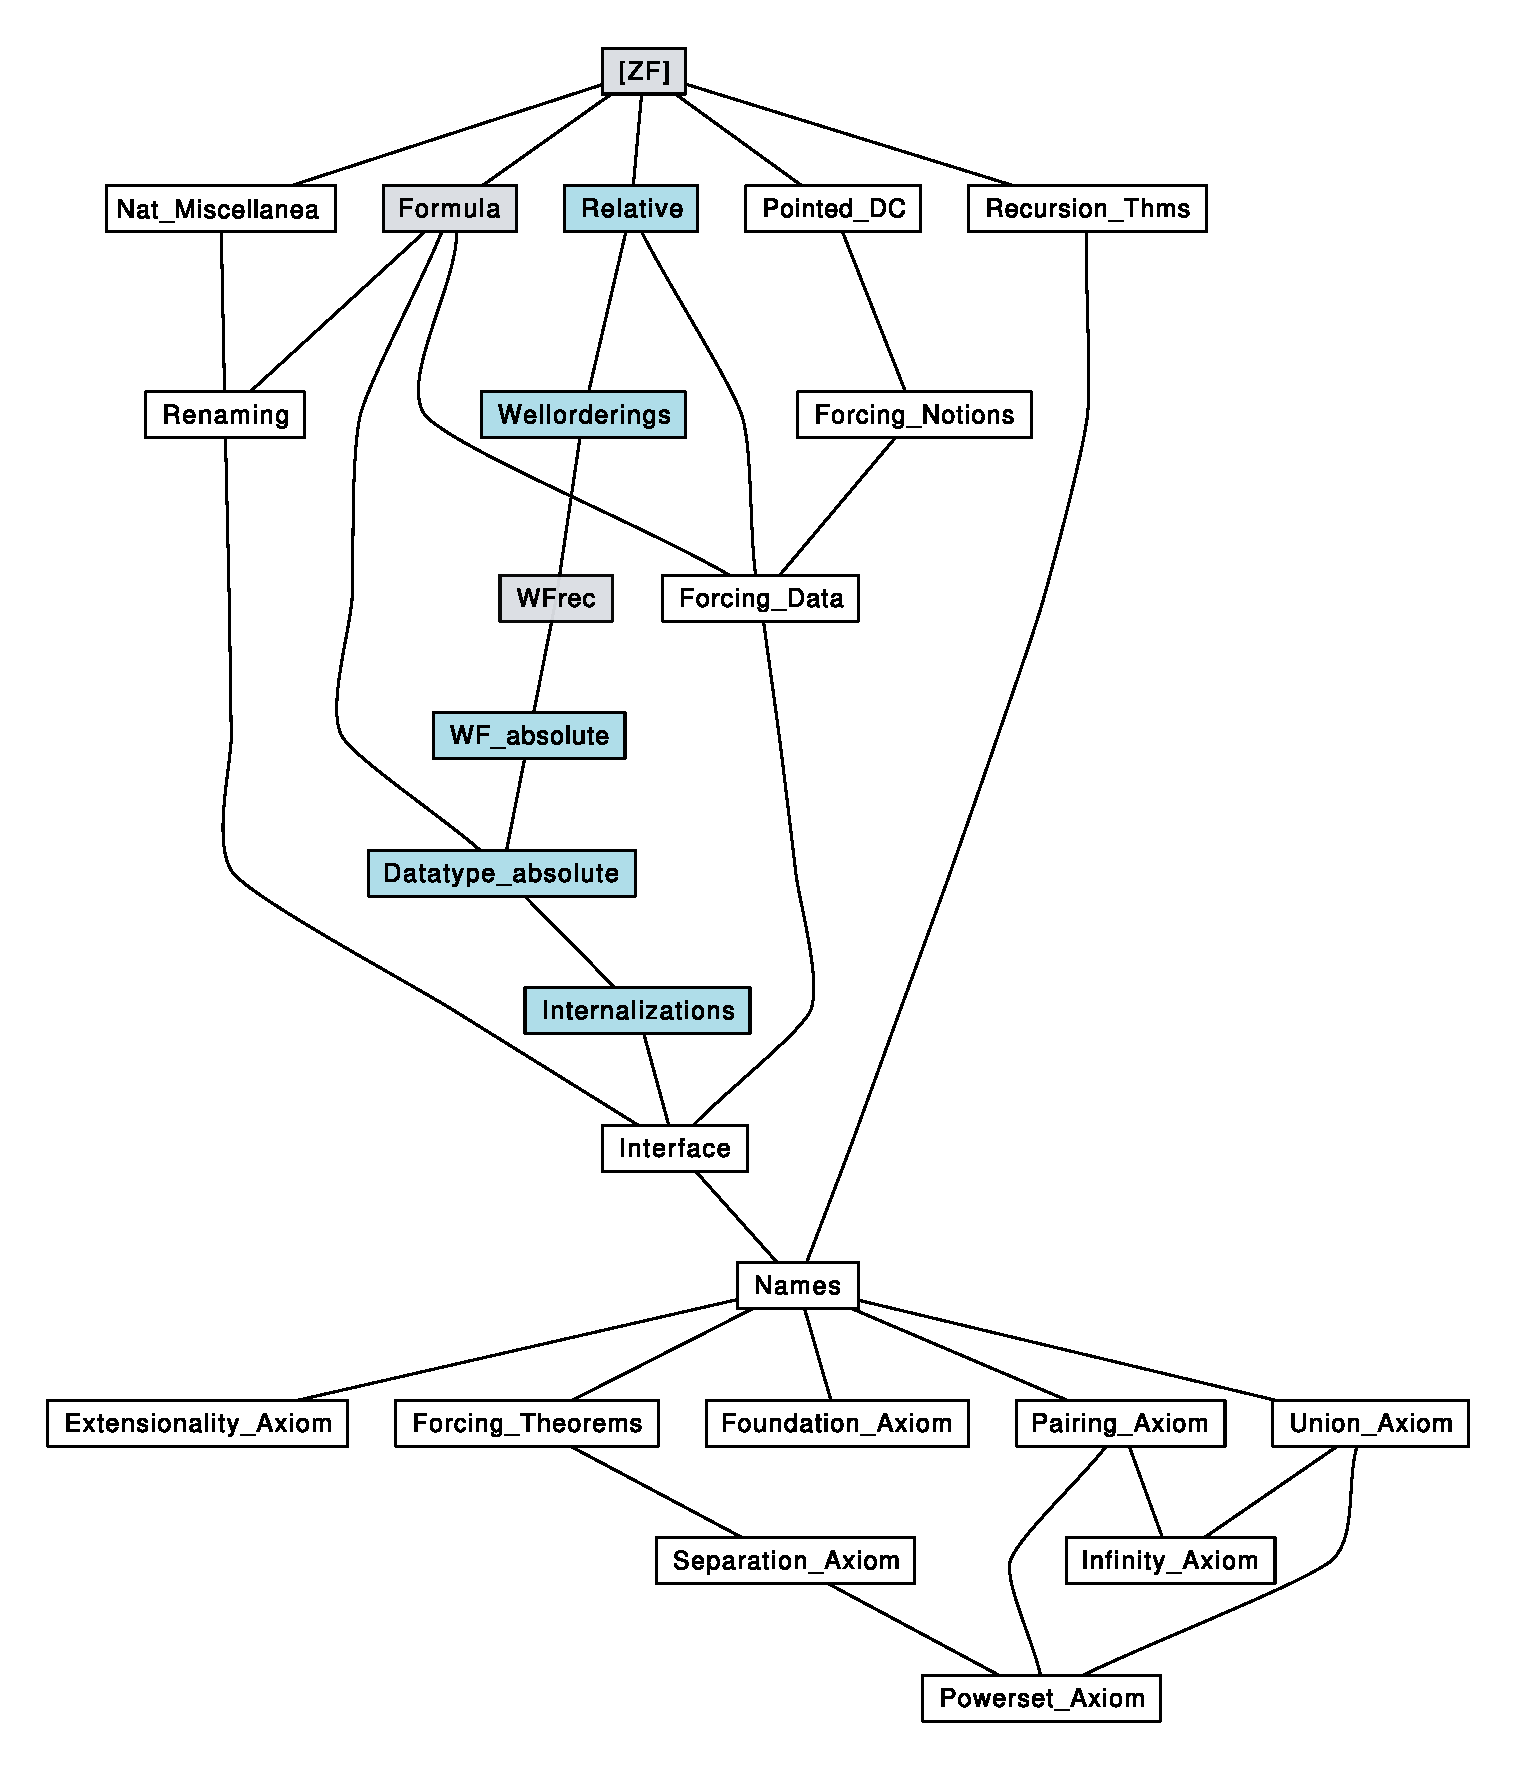
\includepdf{session_graph_colored.pdf}


%%% Local Variables: 
%%% mode: latex
%%% TeX-master: "Separation_In_MG"
%%% ispell-local-dictionary: "american"
%%% End: 
